\documentclass{article}

\usepackage{graphicx}
\usepackage{amssymb}
\usepackage{wasysym}
\usepackage{color}
\usepackage{pgf}
\usepackage{url}
\usepackage{float}
\usepackage{rotating}
\usepackage{dcolumn}
\usepackage{booktabs}
\usepackage[a4paper,inner=20mm, outer=20mm, top=25mm, bottom=20mm,twoside]{geometry}
\usepackage{array}

\usepackage{dcolumn}
\usepackage{booktabs}
\usepackage{longtable}
\usepackage{listings}
\lstloadlanguages{% Check Dokumentation for further languages ...
         %[Visual]Basic
         %Pascal
         %C
         C++	
         %XML
         %HTML
         %Java
 }

\definecolor{dkgreen}{rgb}{0,0.6,0}
\definecolor{gray}{rgb}{0.5,0.5,0.5}
\definecolor{mauve}{rgb}{0.58,0,0.82}

\lstset{
	language=C++,                % the language of the code
	basicstyle=\footnotesize,           % the size of the fonts that are used for the code
	numbers=left,                   % where to put the line-numbers
	numberstyle=\tiny\color{gray},  % the style that is used for the line-numbers
	stepnumber=2,                   % the step between two line-numbers. If it's 1, each line 
												% will be numbered
	numbersep=5pt,                  % how far the line-numbers are from the code
	backgroundcolor=\color{white},      % choose the background color. You must add \usepackage{color}
	showspaces=false,               % show spaces adding particular underscores
	showstringspaces=false,         % underline spaces within strings
	showtabs=false,                 % show tabs within strings adding particular underscores
	%   frame=single,                   % adds a frame around the code
	rulecolor=\color{black},        % if not set, the frame-color may be changed on line-breaks within not-black text (e.g. commens (green here))
	tabsize=2,                      % sets default tabsize to 2 spaces
	captionpos=b,                   % sets the caption-position to bottom
	breaklines=true,                % sets automatic line breaking
	breakatwhitespace=false,        % sets if automatic breaks should only happen at whitespace
	title=\lstname,                   % show the filename of files included with \lstinputlisting;
												% also try caption instead of title
	keywordstyle=\color{blue},          % keyword style
	commentstyle=\color{dkgreen},       % comment style
	stringstyle=\color{mauve},         % string literal style
	escapeinside={\%*}{*)},            % if you want to add a comment within your code
	morekeywords={*,...}               % if you want to add more keywords to the set
	framexleftmargin=17pt,
	framexrightmargin=5pt,
	framexbottommargin=2pt,
}
 
\begin{document}
\title{Measurement of the nuclear modification factor $R_{AA}$ with ALICE}
\author{R.~Averbeck$^1$, F.~Bock$^2$, B.~Doenigus$^1$, Y.~Foka$^1$, 
        P.~Luettig$^3$, S.~Masciocchi$^1$,\\
        K.~Schwarz$^1$, R.~Simon$^1$, J.~Thaeder$^1$\\
\normalsize $^1$Research Division and ExtreMe Matter Institute EMMI,\\
\normalsize GSI Helmholtzzentrum f\"ur Schwerionenforschung, Darmstadt, Germany\\
\normalsize $^2$Physikalische Institut, Ruprecht-Karls-Universit\"at
\normalsize Heidelberg, Germany\\
\normalsize $^3$Institut f\"ur Kernphysik, Goethe University
\normalsize Frankfurt, Germany
}
\maketitle

\tableofcontents

\newpage
\section{Physics Motivation}
\subsection{The ALICE Detector System}
ALICE (A Large Ion Collider Experiment) is one of the four large experiments 
at the CERN Large Hadron Collider. ALICE has been designed to study heavy-ion 
collisions. It also investigates proton-proton (pp) collisions, which primarily
provide reference data for the heavy-ion program but, in addition, allow for a 
number of genuine proton-proton physics studies.

The ALICE detector has been designed to cope with the highest particle 
multiplicities anticipated for collisions of lead nuclei at the extreme 
energies of the LHC. It is composed out of different subdetectors. 
In the Central Barrel these are the Inner Tracking System (ITS), consisting 
out of three high resolution silicon detectors systems featuring two layers 
each, the Time Projection Chamber (TPC), the Transition Radiation Detector 
(TRD), the Time Of Flight detector (TOF), the High Momentum Particle 
Identification Detector (HMPID), two electomagnetic calorimeters EMCal and 
PHOS, and ACCORDE, a dedicated cosmic ray detector. In the following analysis 
mainly the TPC and to some extent the ITS will be used. 

\subsection{Nuclear Modification Factor $R_{AA}$}
In the year 2010, data from the first heavy-ion collisions at the LHC have 
been recorded by the experiments. The ALICE experiment, which is well suited 
for the measurement of the properties of particles in high particle density 
environments, has measured the nuclear modification factor $R_{AA}$ for 
unidentified charged particles. $R_{AA}$ is a measure for the difference in 
particle production in pp and nucleus-nucleus collisions, taking into account 
the different collision geometries. $R_{AA}$ is defined as:
\begin{equation}
R_{AA} = \frac{Y(PbPb)}{\langle N_{coll}\rangle Y(pp)}
\end{equation}
where Y(PbPb) and Y(pp) are the yield (or number of particles per event)
in PbPb and pp collisions, respectively, and $\langle N_{coll}\rangle$ is
the average number of so-called binary nucleon-nucleon collisions, which have 
taken place in the collision of two lead ions. Since each lead nucleus consists
of 208 nucleons, i.e. protons and neutrons, it is clear that a typical Pb-Pb
collisions can be seen as a superposition of many pp collisions. 
$\langle N_{coll}\rangle$, which can be determined in the experiment, measures 
how many pp collisions should be equivalent on average to one Pb-Pb collision.

If the nuclear modification factor is equal to one, the production of 
particles in one Pb-Pb collision on average is the same as in 
$\langle N_{coll}\rangle$ independent pp collisions. Naively, this could
be interpreted such that the physics of pp and Pb-Pb collisions is the
same.

\subsection{Centrality}

\begin{figure}[h]
	\centering
	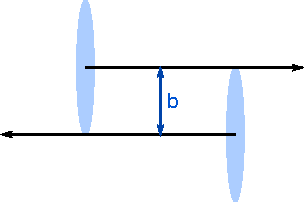
\includegraphics[width=0.45\textwidth]{bParameter.pdf}
 	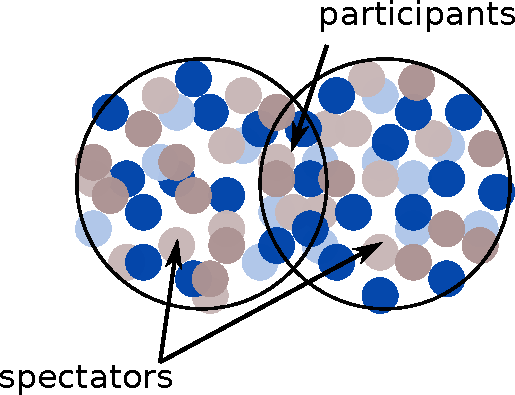
\includegraphics[width=0.45\textwidth]{2Nucleicolliding.pdf}
	\caption{Illustration of two colliding atomic nuclei, indicating the 
                 impact parameter b (left), as well as the the participating 
                 nucleons and the spectators (right).}
	\label{fig:Impactparameter}
\end{figure}

Nuclei of lead atoms are large compared to protons. This results in the fact
that not all Pb-Pb collisions are the same in terms of the collision geometry.
The parameter which controls the geometry in the first place is the so-called
impact parameter $b$, which is the distance of the centers of the two colliding
Pb nuclei in the transverse direction as indicated in the left panel of
Fig.~\ref{fig:Impactparameter}. A collision with small impact parameter b
(which can be as small as zero) is called a central collision, while more
grazing collisions with large b (which can be as large as two times the
radius of the colliding nuclei) is called a peripheral collision. 
In general, the energy density reached in nucleus-nucleus collisions is
larger in central collisions than in perpiheral collisions. If the energy
density becomes large enough a new state of matter, the quark gluon plasma
(QGP) is created. In a QGP, the matter does not consist of protons and 
neutrons any more but the relevant particles that determine the properties
of this phase of matter are the quarks and gluons themselves.

In order to be able to study this phase transition from ordinary nuclear
matter to the QGP one first has to be able to distinguish central and
peripheral collisions from each other, i.e. one has to measure the collision
centrality on an event by event basis. How can this be done? Ideally one
would like to measure directly the impact parameter $b$ but that, 
unfortunately, is not possible.

A quantity that is related to the collision centrality and which can be
measured is the number of particles produced in a collision. In a central
collision essentially all neutrons and protons in the lead nuclei collide
with each other at least ones. They are all so-called participants. Many
collisions of participating protons and nucleons take place and, consequently,
a lot of particles are produced in central Pb-Pb collisions. In contrast,
in more peripheral collisions there is a number of protons and neutrons in 
the colliding lead nuclei which do not fly through the collision zone and,
consequently, do not collide with another proton and neutron. These are the
so-called spectators. Obviously, in a peripheral Pb-Pb collision less
collisions of individual protons and neutrons take place than in a central
Pb-Pb collision and, therefore, less particles are produced. In summary,
the number of produced particles is a good measure for the centrality of a 
collision. The number of participating nucleons $N_{part}$ and the number
of proton-proton like binary nucleon-nucleon collisions $N_{coll}$ they suffer
can be modeled in a so-called Glauber calculation. Without going into any
details, one can say that, with the help of the Glauber model, the measured
number of produced particles with various detectors in the ALICE setup can
be translated into a measure of the centrality of each individual Pb-Pb
collision.

With ALICE it is possible to measure the number of produced particles and, 
via that, the event centrality in a number of ways: via the multiplicities 
measured in the SPD, the VZERO, or the TPC detectors. The correlation of the 
VZERO amplitude, which is a measure of the number of charged particles hitting
the VZERO detectors, and the TPC track multiplicity, which is the number
of tracks reconstructed in one event in the TPC, is shown in the upper panel
of Fig.~\ref{fig:Centrality}. Not surprisingly, these quantities are
nicely correlated.

For the present analysis the centrality measurement will be taken from the
VZERO amplitude. The recorded Pb-Pb collisions are grouped into so-called
centrality classes, which are defined by a minimum and a maximum percentile
of the VZERO amplitude distribution. For example, the centrality class
0-10\% contains those 10\% of all events which have the largest 
VZERO amplitudes and, therefore, are the most central events.
The centrality class 30-40\% also contains 10\% of all the events, but 
30\% of all events have larger VZERO amplitudes (they are more central)
and 60\% of all events have smaller VZERO amplitudes (they are more 
peripheral). 

The lower panel of Fig.~\ref{fig:Centrality} shows the distributions of
the number of charged particle tracks recorded in all collisions independent
of centrality, which is called the minimum bias multiplicity distribution.
In addition, the multiplicity distributions are shown for the most central,
a mid-central, and a peripheral centrality class selected as described above.
As expected, on average events contain more charged particle tracks if they
are more central collisions.

\begin{figure}[t]
	\centering
   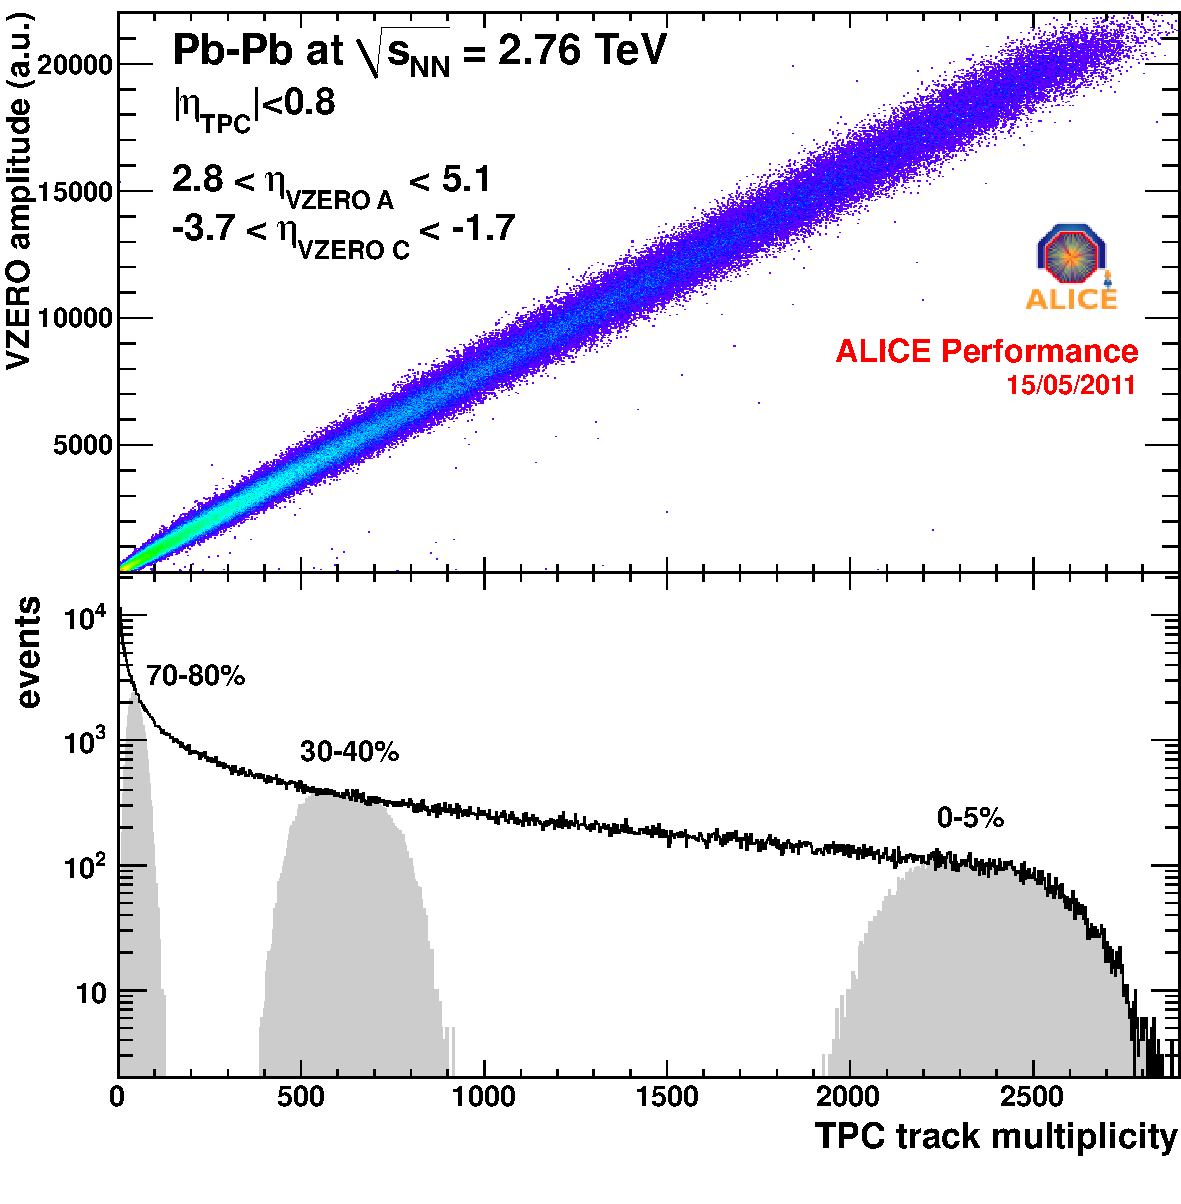
\includegraphics[width=0.48\textwidth]{2011-May-22-tpcv0_combined3only.pdf}
	\caption{Correlation between the VZERO amplitude and the TPC track 
                 multiplicity measured with ALICE (upper panel). Distribution 
                 of the TPC track multiplicity for all (minimum bias) Pb-Pb
                 collisions (histogram) and for the centrality classes 0-5\%,
                 30-40\%, and 70-80\% (grey distributions) as selected by
                 cutting on the VZERO distribution.}
	\label{fig:Centrality}
\end{figure}

For each given centrality class the corresponding number of participating
nucleons $N_{part}$ and the number of binary collisions $N_{coll}$ can be
determined using a Glauber model calculation as mentioned above.

\subsection{$R_{AA}$ as function of the transverse momentum}
For all ecentrality classes the nuclear modification factor $R_{AA}$ can be 
measured as a function of the transverse momentum $p_T$ of charged particles.
$p_T$ is the momentum component of the particle in the $xy$-plane perpendicular 
to the beam axis $z$. It can be calculated:

\begin{eqnarray*}
  p_{T} = \sqrt{p_x^2 + p_y^2}
\end{eqnarray*}

It is an interesting question whether $R_{AA}$ depends on the transverse
momentum of a particle. Charged particle with large $p_T$ typically originate
from violent scattering processes of quarks or gluons in the incoming nuclei
(called hard processes). These quarks or gluons propagate through the hot and
dense medium produced in the collision and they interact with this medium.
This interaction, in general, will lead to energy loss of the fast moving
quark or gluon and that could leave its footprint on $R_{AA}$.

Clearly, one would expect that for the most peripheral collisions, i.e.
the centrality class 70-80\% in the current case, $R_{AA}$ is close to one
because a peripheral Pb-Pb collision should not be too different in terms
of particle production from a pp collision. To find out what happens in
more central collisions is the purpose of the current analysis.

\section{Visual Analysis}
\subsection{The Task}
The goal of this visual analysis is to make you familar with the concepts of:

\begin{itemize}
\item \textit{clusters}: electronic signature left by a particle traversing a 
  detector, with additional information about time or space
\item \textit{track}: Path of a praticle trough the detectorssystem, 
  reconstructed on the basis of the space and time information of individual 
  clusters. The path of the particle is straight in an environment without 
  additional forces (i.e. no magnetic (B) or electric fields (E)). If a charged
  particle is traversing a magnetic field it will be influenced by the magnetic
  field due to the Lorentz force and the tracks will be curved. 
\item \textit{primary vertex}: collision vertex selected for the analysis
\item \textit{sattelite collisions/pile-up vertices}: not selected collisions 
  vertices seen in the detector due to high intensity of the LHC-beam
\item \textit{primary track}: track orginating from the selected collision 
  vertex (for this analysis: distance of closest approach $<$ 1 cm)
\item \textit{secondary track}: track not orginating from the primary vertex 
  but from a secondary decay vertex (for example strange particle decays)
\end{itemize}

Furthermore your task will be to count for the 30 pp events at center of mass 
energy ($\sqrt{s}$) $= 2.76$ TeV at a magnetic field of 0.5 T the number of 
tracks originating from the primary vertex (\textit{multiplicity}) by clicking 
on each primary tracks. The tool will count for you the total number of tracks 
in an event and will publish it to a histogram, from which you then can read 
of the mean of the distribution after having analysed the 30 events. 
Additionally you should count the multiplicity in one peripheral, one 
semi-central and one central Pb-Pb event and calculate an integrated $R_{AA}$ 
for these events.

For the integrated $R_{AA}$ calculation you need to divide the number of
charged particle tracks in the three Pb-Pb events by 0.6 (why?) by the 
number of binary collisions $N_{coll}$ as given in Table~\ref{tab:nCollVisual}.

\begin{table}
  \centering
  \begin{tabular}{llr}
    \toprule
    Classification & centrality class & $N_{coll}$ \\ \midrule
    peripheral 	& 80 - 90 \% & 6.32 \\
    semicentral & 20 - 40 \% & 438.80 \\
    central & 0 - 5 \%	& 1686.87 \\ \bottomrule
  \end{tabular}
  \caption{Classification of the Pb-Pb events for the visual analysis and 
           their corresponding number of binary collisions $N_{coll}$ according 
           to the Glauber model.}
  \label{tab:nCollVisual}
\end{table}

\subsection{The Tool}
For this purposes a software has been developed based on the ROOT  
(\url{http://root.cern.ch/}). This software tool can visualize the clusters 
in the main detectors of the central barrel (ITS, TPC, TRD and TOF) and show 
the reconstructed tracks which pass some general quality cuts. Furthermore, it 
can show you the primary vertex and the primary tracks originating from this 
vertex and it will help you count them. The tool can be started from a terminal
in the directory MasterClass2012/Part1 with the command:

\begin{lstlisting}[]
 	root masterclass.C
\end{lstlisting}

The window shown in Fig. \ref{fig:Startup} will pop up and, in addition, you 
will see a short version of the instructions.

\begin{figure}[b]
 	\centering
 	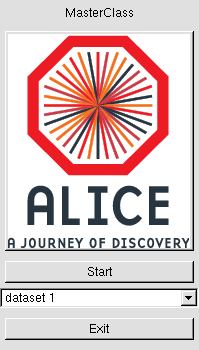
\includegraphics[width=0.2\textwidth]{StarterMasterClasses.png}
	\caption{Startup window for the ALICE master class.}
	\label{fig:Startup}
\end{figure}

There are three things which you can do:
\begin{itemize}
\item Start - the analysis.
\item Select the data set which you would like to analyse (the selection 
      field). Please ask your tutor which data set you should be taking.
\item Exit - finish the analysis.
\end{itemize}

\begin{figure}
  \centering 
  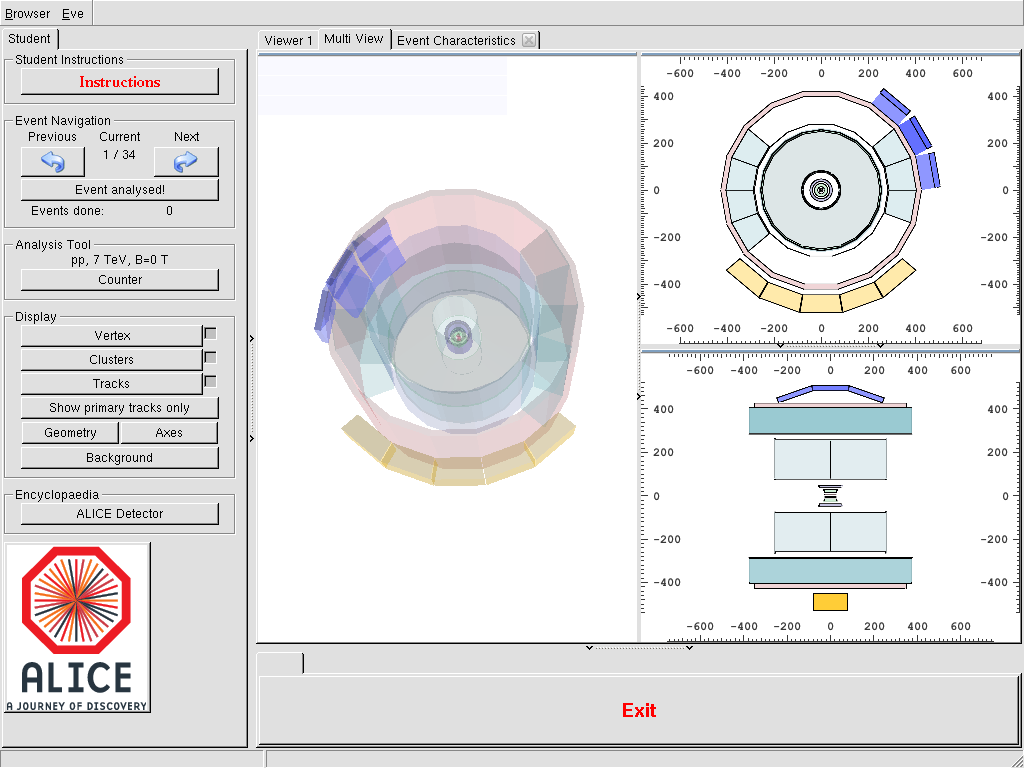
\includegraphics[width=\textwidth]{EVEMainWindow.png}
  \caption{Main window for the visual analysis directly after start-up}
  \label{fig:EVE}
  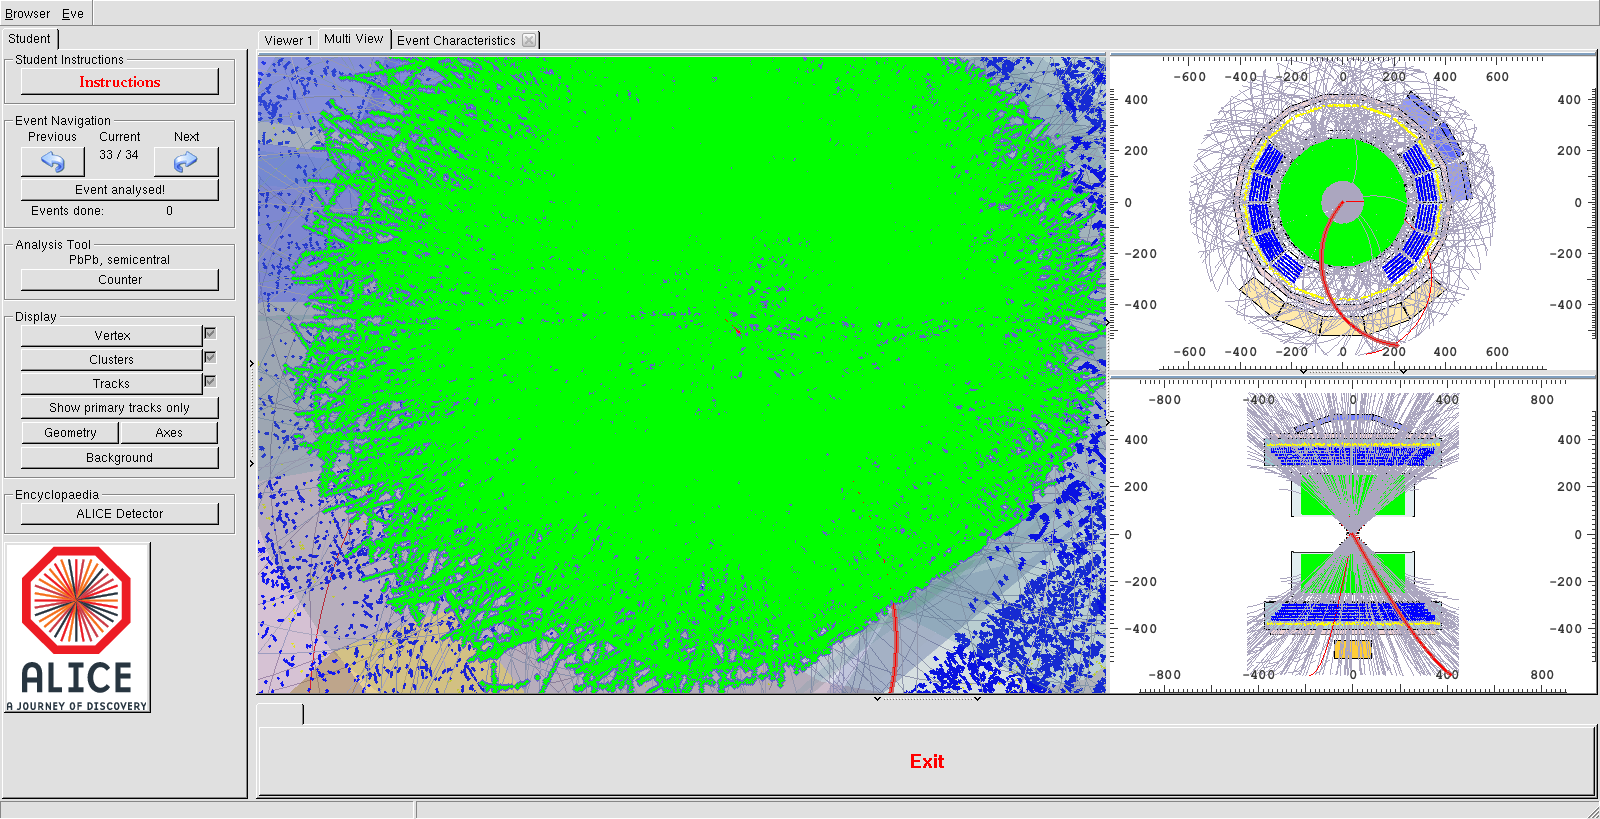
\includegraphics[width=\textwidth]{PbPbEventinTheEVEdisplay.png}
  \caption{Pb-Pb event seen in the Master Class visualisation tool.}
  \label{fig:PbPbEvent}
\end{figure}

After having pressed the button ``Start'', it will take a moment, due to 
compiling, until the window shown in Fig. \ref{fig:EVE} will pop up with a 
shorter version of the full instructions for the visual analysis.\\

This window is divided into two main sections: a left column with the options 
and a right bigger column with the event display. You can see at the top three
different tabs ``Viewer 1'', ``Multi View'', and ``Event Characteristics''.
The first two of them are event displays. ``Viewer 1'' allows you to see the 
event in 3D as a single view, while the ``Multi View'' already presents it to 
you in two projections ($r\phi$ projection: right upper corner, and 
rz projection: right lower corner) and in the 3D-view in the middle.	
In the event display you can click on anything you want and can navigate 
either with the mouse by holding the right mouse botton (turning the 3D-view), 
or by just using the arrows on your keyboard. To zoom in or out please click in
the corresponding view and use the ``+'' or ``-'' keys on your keyboard. By 
clicking on the tracks you can count them for you multiplicity distribution, 
if the counter is open. In addition, several properties of the track will be 
displayed in the upper part of the counter. If you have clicked on a track it 
turns red. However, if you change something in your display settings, e.g. 
switching on and off the tracks it will be shown in grey/blue again.

For counting the primary tracks please select the ``Show primary tracks only''
button first, it will make your life much easier. In case of Pb-Pb events you 
should probably turn the clusters off as it will take a lot of time otherwise 
and you will not see anything anymore. In Fig. \ref{fig:PbPbEvent} you can see 
a semicentral Pb-Pb event with everything switched on. The multiplicities in 
the three Pb-Pb events need to be written down on the prepared sheet of paper, 
as they will not be stored anywhere.

\begin{figure}
  \centering 
  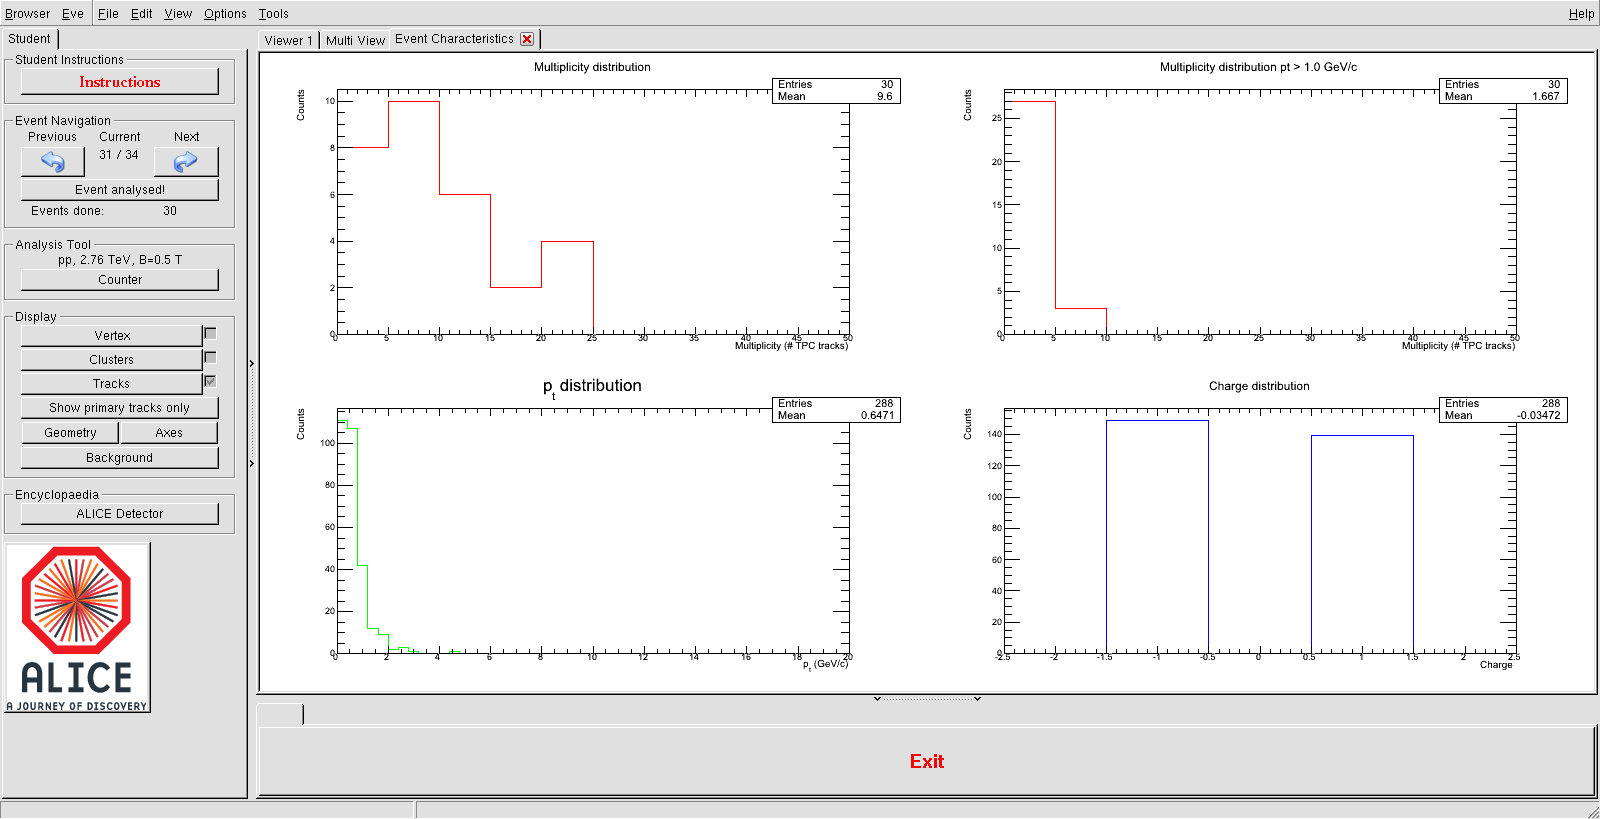
\includegraphics[width=\textwidth]{HistogramsEventChar.png}
  \caption{Histograms for the event and track characteristics for pp events at 
    $\sqrt{s} = 2.76$ TeV.}
  \label{fig:EventHistos}
\end{figure}

In the ``Event Characteristics'' tab  (Fig. \ref{fig:EventHistos}) you can see 
four histograms. These will be filled for pp at $\sqrt{s} = 2.76$ TeV only. 	
The left column of the main window offers the following options:

\begin{itemize}
\item Instructions:\\
  This button will again display the shorter version of these instructions.
\item Event navigation:\\
  You can navigate between the different events with ``next'' and ``previous''
  while the current event number will be displayed in the middle. 
  If you click on the ``Event analysed'' button the multiplicity will be 
  published to the corresponding histogram. (will be explained later)
  In addition, this will increase the number of analysed events in the row 
  below the button.
\item Analysis Tool:\\
  In this part you can start the counting tool according to the event type 
  being analysed. There are 5 different types of the events:
  \begin{itemize}
  \item 1 pp event at $\sqrt{s} = 7$ TeV with zero magnetic field
  \item 30 pp events at $\sqrt{s} = 2.76$ TeV with a magnetic field of $B= 0.5$ T
  \item 1 peripheral Pb-Pb event (32$^{nd}$ event)
  \item 1 semi-central Pb-Pb event (33$^{rd}$ event)
  \item 1 central Pb-Pb event (34$^{th}$ event)
  \end{itemize}
  \begin{figure}
    \centering
    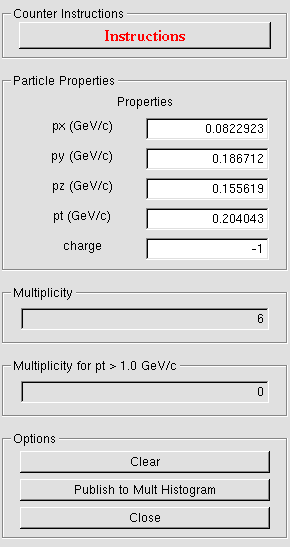
\includegraphics[width=0.35\textwidth]{CounterNormalPP.png} \hspace{0.5cm}
    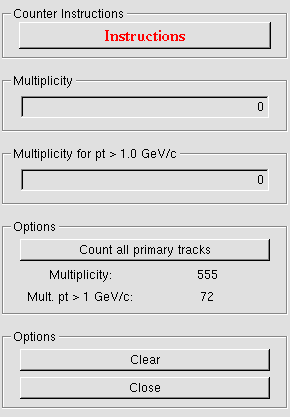
\includegraphics[width=0.35\textwidth]{CounterPbPb.png}
    \caption{Counting tool for pp (left) and Pb-Pb (right) collisions.}
    \label{fig:Counter}
  \end{figure}
  Please close the previous counter if the event type changes and open a new 
  one by clicking on the button ``Counter''. The two different types shown in 
  Fig.~\ref{fig:Counter} will show up according to the chosen collision 
  conditions. For the first class of events ($B= 0$ T) there exists no 
  counting tool. In both counters some properties either of the tracks or the 
  event in total can be displayed, like $p_x, p_y, p_z, p_t,$, charge for 
  tracks, or multiplicity for the event. The modes are slightly different for 
  the different counters. In case of pp (2.76 TeV, B= 0.5 T) the $p_{T}$ and 
  charge will be automatically published to the histograms in the tab 
  ``Event Characteristics''. The multiplicities in this case can be either 
  published by the clicking the button ``Event analysed'' in the main window 
  or by pressing ``Publish to Mult Histogram''. This should only be done if 
  you are sure you counted really all primary tracks, as this is not reversable
  and will screw up your mean multiplicity otherwise. The ``Clear'' button 
  resets all entries to zero. However, all track properties which have already 
  been published will remain in the histograms. For the Pb-Pb case there exists
  the possibilty of automatically counting the primary tracks. Please reduce 
  the tracks to the primary tracks only before (Clicking button ``Show primary 
  tracks only'' in the main window). For Pb-Pb there exists no automatic 
  storing of the multiplicities. Therefore, please keep track of these yourself
  on a sheet of paper.
\item Display:\\
  This part allows you to switch on and off several features of the event 
  display (like primary vertex - ``Vertex'', clusters - ``Clusters'', 
  tracks - ``Tracks'', geometry of the detectors -``Geometry'', coordinate 
  axis - ``Axis'' and change the background color ``Background''). Furthermore,
  it allows you to reduce the tracks to the tracks originating from the 
  primary vertex by pressing ``Show primary tracks only''. If you press it 
  twice it will return to the full number of good tracks in the event.
\item Encyclopaedia:\\
  In this section you can learn a little more about the ALICE detector.
  Furthermore, information about the individual detectors will pop up by 
  clicking at the detector volumes in the event display. If you want to close 
  this again just click in the window.
\end{itemize}

\section{The Large Scale Analysis}
\subsection{The Task}
In this part of the ALICE master class you will be introduced to a large scale 
analysis based on real Pb-Pb data. Your task will be to implement the 
extraction of the Pb-Pb transverse momentum spectra in a given centrality 
class from a prepared data sample (called a tree), which contains the 
centrality of the event, the track multiplicity, and the transverse momentum 
of each track. Furthermore, you are supposed to write a simple program which 
calculates the $R_{CP}$ (what's that? ask your tutor!) and $R_{AA}$ and plots 
the transverse momentum spectra, the track multiplicity, the $R_{CP}$ and 
$R_{AA}$ for different centralities in one plot. 

\subsection{Building the Transverse Momentum Spectra}

For this part of the analysis you need to program approximately 10-15 lines of 
code in a prepared ROOT macro. The macro is called 
``AnalyseTreeForRAAStudents.C'' and can be found in the folder 
MasterClasses2012/Part2. It can be started with the command in this directory:

\begin{lstlisting}[]
root -x -q -b -l 'AnalyseTreeForRAAStudents.C++("MasterClassesTree_LHC10h_Run139036.root","PbPb","kFALSE",0,5)'
\end{lstlisting}

The options after the ROOT call (``-x -q -b -l'') are some settings for 
running root in quiet mode and executing the macro which is following 
afterwards. The real function call follows. First, there is the name of the 
macro ``AnalyseTreeForRAAStudents.C''. Then the ``++'' stands for compiled 
mode and afterwards several options are given to the macro itself. 

\begin{itemize}
\item[1] filename $=$ "MasterClassesTree\_LHC10h\_Run139036.root"\\
  This is the name of the file you would like to analyse.
\item[2] collision system =  "PbPb" \\
  This is the selected collision system which you will be analysing, in your 
  case this will always be "PbPb".
\item[3] test mode = "kFALSE"\\
  If you set this variable to "kTRUE" the macro will be run in test mode and 
  only 1000 events and 1000 tracks are processed. This makes the execution
  much faster.
\item[4] start of centrality class = 0\\
  This variable determines the starting value of your centrality class.
\item[5] end of centrality class = 5\\
  This variable determines the end value of your centrality class. 
  In this example the most central bin from 0 to 5\% will be analysed.
 \end{itemize}

The macro is structured as follows:

First there are two functions to make the plots look nicer 

\begin{lstlisting}[]
void StyleSettings() 
void HistoSetMarkerAndColor( TH1* histo1, Style_t markerStyle, Size_t markerSize, Color_t markerColor, Color_t lineColor )
\end{lstlisting}

These two you should not modify however you should read the comments above 
them to get an idea how to use them. Comments in ROOT/C++ are starting with 
``//'' or the look like this: ``/* ---- text ----*/''. Comment statements will 
never be executed. Afterwards the main function starts. It has the same name 
as the macro itself just without the ''.C`` in the end. The code belonging to 
a function is always within these brackets \{ \}. The same is true for loops 
or conditional statements. 

\begin{lstlisting}[]
 	void AnalyseTreeForRAAStudents(TString filename = "MasterClassesTree_LHC10h_Run139036.root", TString optionCollSystem = "PbPb", TString optionTest= "kFALSE", Int_t startCentrality = 0., Int_t endCentrality = 100.)
\end{lstlisting}

The options of the main function are already explained above. Here, just the 
variable names and the standard settings are given in addition.

In this main function the first task is to attach the file with the input and 
set the correct variable names

\begin{lstlisting}[firstnumber=130]
//*********************************************************************************
//Declaration of leaves types for track tree 
//*********************************************************************************
Float_t         trackCentrality;  // variable for the centrality in the track tree
Double_t        trackPt;			// variable for the transverse momentum of the track

//*********************************************************************************
//Declaration of leaves types for event tree
//*********************************************************************************
Float_t         eventCentrality;	// variable for the centrality in the event tree
Int_t           eventMult;			// variable for the multiplicity in the event
\end{lstlisting}

Afterwards these are related to the quantities in the corresponding parts of 
the input tree (Line 142 - 155) and the number of entries in each tree is 
evaluated (Line 161 - 183). Then the binning in transverse momentum is 
determined and the histograms are created.

\begin{lstlisting}[firstnumber=185]
//*********************************************************************************
// Definition of bins in transverse momentum pt, due to steply falling spectrum 
// and not enough statistics at high pt 
//*********************************************************************************
Int_t fNBinsPt = 54; 								 
Double_t fBinsPt[55] = 	{0, 0.05, 0.1, 0.15, 0.2, 0.25, 0.3, 0.35, 0.4, 0.45,
								0.5, 0.55, 0.6, 0.65, 0.7, 0.75, 0.8, 0.85, 0.9, 0.95,
								1, 1.1, 1.2, 1.3, 1.4, 1.5, 1.6, 1.7, 1.8, 1.9,
								2, 2.2, 2.4, 2.6, 2.8, 3, 3.2, 3.4, 3.6, 3.8,
								4, 4.5, 5, 5.5, 6, 6.5, 7, 8, 9, 10, 
								11, 12, 13, 14, 15};
								
								
								
//*********************************************************************************
// Defintion of histograms:
// * to be filled with trackpt and number of charged tracks in the TPC (TH1*)
// * correlation between centrality an nTracks TPC (TH2F)							 
//*********************************************************************************	
								
TH1D *htrackPt = new TH1D("htrackPt","track pt",fNBinsPt,fBinsPt);
TH1F *hNTPC = new TH1F("hNTPC","Number of TPC tracks ",200,0,2000);
TH2F *hNTPCvsCent = new TH2F("hNTPCvsCent","Number of TPC tracks ",200,0,2000, 100, 0, 100);

//*********************************************************************************
// Definition of correction histogram in order to normalise for the binwidth in
// Pt
//*********************************************************************************
TH1D* fDeltaPt = new TH1D("deltaPt","",fNBinsPt,fBinsPt);
for(Int_t iPt=1;iPt<fNBinsPt+1;iPt++){
	fDeltaPt->SetBinContent(iPt,fBinsPt[iPt]-fBinsPt[iPt-1]);
	fDeltaPt->SetBinError(iPt,0);
}
\end{lstlisting}

After that, the event quantities are read from the event tree and filled in 
the corresponding histograms. To accomplish that a loop over all entries in 
this tree has to be created (line 230) and for each event one has to check 
whether it belongs to the correct centrality class (line 232). The lines 233 
and 234 fill the one and two dimensional histograms for the number of tracks 
(versus centrality).

\begin{lstlisting}[firstnumber=219]
 	//*********************************************************************************
	// * Reading the entries form the event tree (extract nTracksTPC) and filling 
	//   it in the multiplicity histograms (hNTPC,hNTPCvsCent)
	// * Distinction between PbPb and pp as for PbPb you need to fill them with 
	//   restriction in centrality
	// * nEntriesPerCent will give you the normalization value for the different 
	//	  centralities
	//*********************************************************************************

	ULong_t nEntriesPerCent= 0;
	ULong64_t nbytes2 = 0;
	for (ULong_t i=0; i<nEntriesEvent;i++) {
		nbytes2 += Event->GetEvent(i);
		if (eventCentrality > startCentrality && eventCentrality < endCentrality){
			hNTPC->Fill(eventMult);
			hNTPCvsCent->Fill(eventMult,eventCentrality);
			nEntriesPerCent++;
		}
		// give an output for every 10Mio events processed to see that is working 
		if ( i%10000000 == 0 ) {
			cout << i/10000000 << " * 10^7 events have been processed" << endl;
		}
	}
\end{lstlisting}

A similar loop has to be created for the track tree as the ''/// To do: `` in 
line 254 indicates. Afterwards the filled histograms need to be plotted and 
saved. For the plotting an example is given in lines 269 - 300, and a similar 
plot should be produced for the transverse momentum as indicated in line 312. 
Please don't forget to uncomment the lines 315-319. Otherwise the scaling will 
not be done correctly. Also, line 341 needs to be uncommented to save the 
histogram in a file. 

\subsection{Building the $R_{AA}$ and $R_{CP}$}
For this part of the analysis you need to program approximately the same amount
of code as in the exercise before. Again a ROOT macro gives you a starting
point. The macro is called ``BuildRAAStudents.C'' and can be found in the same 
directory as the previous one. It can be started by running the following 
command in this directory:

\begin{lstlisting}[]
root -x -q -b -l 'BuildRAAStudents.C++("RAABaseOutput.root")'
\end{lstlisting}

As already described in the previous section, the first commands are just some 
ROOT settings. The macro name follows, which should be executed in compiled 
mode as the ``++'' indicates. The only option which you can hand over is the 
file name of the input file for the Pb-Pb results, which were produced in the 
previous exercise. This file will contain the results for different 
centralities. You just need to find out how to read them from the file.

The first part in the macro ``BuildRAAStudents.C'' contains again the 
functions for the styling of the plots. Then follows the main-routine: 

\begin{lstlisting}[firstnumber=101]
void BuildRAAStudents(TString filename = "RAABaseOutput.root")
\end{lstlisting}

In this function the first few lines are for general setting. Then follows the 
definition of the variable for the number of collisions in each centrality, 
$nColl\_0\_5$, where the first number indicates the start centrality and the 
second one the end of the centrality bin (lines 111-123).

Afterwards the Pb-Pb and pp spectra are read from the corresponding files and 
scaled to the number of binary collisions. Here you need to add the other 
centrality classes as indicated in line 132 and 140. The pp spectrum gives you 
the baseline for the $R_{AA}$. 

\begin{lstlisting}[firstnumber=125]
 	//*********************************************************************************
	//Attaching & reading the input-file
	//*********************************************************************************   
	TFile fileInput(filename.Data());  
	//____ reading the number of TPC tracks for pp events & 0-5% PbPb events___________
	TH1D *hNTracksTPCPbPb_0_5 =			(TH1D*)fileInput.Get(Form("nTracksTPC_PbPb_%i-%i",0,5));
	TH1D *hNTracksTPCPbPb_70_80 =			(TH1D*)fileInput.Get(Form("nTracksTPC_PbPb_%i-%i",70,80));
	/// To do: Do the same for the other centralities 
	
	//_____reading the pt-spectrum for 0-5% & 70-80% PbPb events, scaling it___________
	//_____by corresponding number of Collisions (nColl)_______________________________
	TH1D *hTrackPtPbPb_0_5 =			(TH1D*)fileInput.Get(Form("trackPt_PbPb_%i-%i",0,5));
	hTrackPtPbPb_0_5->Scale(1./nColl_0_5);
	TH1D *hTrackPtPbPb_70_80 =			(TH1D*)fileInput.Get(Form("trackPt_PbPb_%i-%i",70,80));
	hTrackPtPbPb_70_80->Scale(1./nColl_70_80);
	/// To do: Do the same for the other centralities 
	
	//*********************************************************************************
	// Attaching and Reading pp-reference file
	//*********************************************************************************   
	TFile* fileInputPP = 		new TFile("PP_2760GeV_BaseLine.root");
	TH1F *hNTracksTPCpp = 		(TH1F*)fileInputPP->Get("nTracksTPC_pp");	
	TH1D* hTrackPtpp = 			(TH1D*)fileInputPP->Get("trackPt_pp");	
\end{lstlisting}

Then the $R_{CP}$ is calculated from the most central (0-5\%) and the most 
peripheral bin (70-80\%). Therefore, you need to divide the most central 
spectrum scaled with $N_{coll}$ by the most peripheral spectrum scaled with the
corresponding $N_{coll}$. As seen in lines 149 ff, this should be done in a 
similar manner for the other centralities and the $R_{AA}$ where the pp 
reference is used as divisor (``To do'' in line 161).

\begin{lstlisting}[firstnumber=149]
	//*********************************************************************************
	// Building the RCP
	//*********************************************************************************
	TH1D*	hRCP_0_5 = (TH1D*)hTrackPtPbPb_0_5->Clone("RCP_vs_Pt_0-5");
	hRCP_0_5->Sumw2();
	hRCP_0_5->Divide(hTrackPtPbPb_70_80);
	/// To do: Do the same for the other centralities 
\end{lstlisting}

The lines 166 to the end then just contain the routines for plotting as 
already explained in the previous section. Here, you should add the other 
centralities as well as the plot for the $R_{AA}$. Don't forget to put the 
axis labels as well as the legends. An example for the legend is given in 
line 189ff.

\end{document}
